\documentclass[a4paper,12pt, oneside]{article}

\usepackage[in]{fullpage}

\usepackage[utf8]{inputenc}
\usepackage[T1]{fontenc}
\usepackage[french]{babel}

\usepackage{amsmath}
\usepackage{amssymb}
\usepackage{mathtools}
\usepackage[inline]{enumitem}
\usepackage[squaren,Gray]{SIunits}
\usepackage{sistyle}
\usepackage[autolanguage]{numprint}
\usepackage{xfrac}
\usepackage{bm}
\usepackage{color}
\usepackage[version=3]{mhchem}
\usepackage{multirow}

\newcommand{\diff}[1]{\mathrm{d}#1}

\let\oldvec\vec
\renewcommand{\vec}[1]{\oldvec{\bm{#1}}}
\newcommand{\uvec}[1]{\hat{\bm{#1}}}

\newcommand{\TODO}[1]{\colorbox{red}{\textbf{\textsc{TODO: #1}}}}

\newcommand{\e}[1]{\ensuremath{\cdot 10^{#1}}}


%opening
\title{Project 3: First report}
\author{Group 1254}
\date{1st of October, 2014}

\begin{document}

\maketitle

\tableofcontents

\section*{Introduction}
%\addcontentsline{toc}{section}{\protect\numberline{}Introduction}
\addcontentsline{toc}{section}{Introduction}

We were asked to answer a series of questions about the mass production of ammonia in a chemical plant. Those questions were:
\begin{enumerate}
 \item what are the quantities of nitrogen and hydrogen needed to produce $\unit{1000}{\ton}$ of ammonia per day?
 \item what is the flow rate of water necessary to maintain the reaction at $\unit{500}{\kelvin}$, knowing that the water enters the reactor at $\unit{25}{\celsius}$ and leaves at  $\unit{90}{\celsius}$?
 \item how are the nitrogen and hydrogen used in the reaction going to be produced?
\end{enumerate}

%\documentclass{article}

%\usepackage[utf8]{inputenc}
%\usepackage[T1]{fontenc}      
%\usepackage[francais]{babel}
%\usepackage{graphicx}
%\usepackage{circuitikz}
%\usepackage[squaren, Gray]{SIunits}
%\usepackage{sistyle}
%\usepackage[autolanguage]{numprint}
%\usepackage{pgfplots}
%\usepackage{amsmath,amssymb,array}
%\usepackage{url}
%\usepackage[version=3]{mhchem}
%\usepackage{array} 

%\begin{document}
%%%%%% titlepage.tex %%%%%%


%\begin{titlepage}
%
%\begin{center}
%
%\textsc{\Large Université Catholique de Louvain}\\[0.5cm]
%\textsc{\Large \'Ecole Polytechnique de Louvain}\\[1cm]
%
%{\Huge \bfseries Projet}\\[0.15cm]
%
%%%\begin{center}
%%%\includegraphics[width = 8cm]{./titlepage/BARRA.jpg}
%%%\end{center}
%
%\rule{\linewidth}{0.3mm}\\[0.1cm]
%{\huge \bfseries Rapport de tache 1}\\[0.02cm]
%\rule{\linewidth}{0.3mm}\\[0.5cm]
%
%{\LARGE \bsc{Groupe} 1}\\[1cm]
%
%\begin{minipage}{0.5\textwidth}
%\begin{flushleft} \Large
%\emph{Auteurs:}\\
%\Large Simon \textsc{Boigelot} \normalsize 75971300\\
%\Large Virgile \textsc{Goyens} \normalsize 83391300\\
%\Large Corentin \textsc{Joachim} \normalsize 75971300\\
%\Large Xavier \textsc{Lambein} \normalsize 54621300\\
%\Large Edward \textsc{Nicol} \normalsize 27101300\\
%\Large Léa \textsc{Paulus} \normalsize 48251100\\
%\Large Abbas \textsc{Sliti} \normalsize 75971300
%\end{flushleft}
%\end{minipage}
%\begin{minipage}{0.4 \textwidth}
%\begin{flushright} \large
%\emph{Cours:} \\
%LFSAB1503\\
%\emph{Professeurs responsables:} \\
%J. De Wilde \\
%P. Luis Alconero \\
%D. Mignon \\
%\emph{Assistant:} \\
%*** \\
%\end{flushright}
%\end{minipage}
%
%\vfill
%
%%%\begin{minipage}{0.3\textwidth}
%%%\begin{flushleft}
%%%\includegraphics[height=2.5cm]{./titlepage/logo-ucl.jpg}
%%%\end{flushleft}
%%%\end{minipage}
%\begin{minipage}{0.3\textwidth}
%\begin{center}
%{\large FSA12BA}\\
%{\large 21 septembre 2014}
%\end{center}
%\end{minipage}
%%%\begin{minipage}{0.3\textwidth}
%%%\begin{flushright}
%%%\includegraphics[height=1cm]{./titlepage/logo-epl.jpg}
%%%\end{flushright}
%%%\end{minipage}
%
%\end{center}
%
%\end{titlepage}


\section{Bilan de masse}

L'équation de la production d'ammoniac selon le procédé Haber-Bosch est la suivante: 

\[
  \ce {N2 + 3H2 -> 2NH3}
  \text.
\]

%Nous voulons calculer la quantité de réactifs pour obtenir une quantité de \unit{1000}{\tonne} d'ammoniac. Pour cela avec les masses molaires respectives de \unit{28}{\gram/\mole} et \unit{2}{\gram/\mole} du diazote et du dihydrogène, il nous faut: 
%\begin{center}
% \begin{tabular}{|l|c|r|}
%   \hline
%    & dihydrogène & diazote \\
%   \hline
%   Nb mole & $88.2\cdot 10^6$ & $29.4\cdot 10^6$ \\
%   Poids & \unit{176.8}{\tonne} & \unit{823.2}{\tonne}  \\
%   \hline
% \end{tabular}
%\end{center}
%=======
Nous voulons calculer la masse de réactifs nécessaire pour obtenir une quantité de \unit{1000}{\tonne}  d'ammoniac. Pour commencer, nous allons déterminer le nombre de moles d'ammoniac produites à l'aide de la masse molaire du composé, qui est de \unit{17}{\gram\per\mole}.
>>>>>>> a7ef90b238d236fb62401147b0a16483fbc9c4f4

\[
  n_\ce{NH3} = \frac {m_\ce{NH3}} {M_\ce{NH3}} = \frac {\unit{10^9}{\gram}} {\unit{17}{\gram/\mole}} = \unit{5.882\e7}{\mole}
  \text.
\]

Ensuite, en utilisant l'équation de réaction, nous pouvons déterminer la quantité de dihydrogène et de diazote nécessaire :

\[
  n_\ce{H2} = \frac{3}{2} n_\ce{NH3} \quad\text{et}\quad n_\ce{N2} = \frac{1}{2} n_\ce{NH3}
  \text.
\]

Enfin, avec les masses molaires des réactifs, respectivement \unit{2}{\gram\per\mole} et \unit{28}{\gram\per\mole} pour le dihydrogène et le diazote, nous obtenons le bilan de masse suivant :

\begin{center}
  \begin{tabular}{llrr}
    & & \multicolumn{1}{c}{\bfseries Moles} & \multicolumn{1}{c}{\bfseries Masse} \\
    \hline
    \multirow{2}{*}{\bfseries Réactifs}
     & \ce{H2} & \unit{8.823\e7}{\mole} & \unit{176.5}{\tonne} \\
     & \ce{N2} & \unit{2.941\e7}{\mole} & \unit{823.5}{\tonne} \\
    \hline
    \bfseries Produits
     & \ce{NH3} & \unit{5.882\e7}{\mole} & \unit{1000.0}{\tonne}
  \end{tabular}
\end{center}

\section{Aspect thermique}

Nous devons faire en sorte que notre réacteur soit à une température constante de \unit{500}{\celsius}. Étant en présence d'une réaction exothermique, pour le refroidir, nous disposons d'un flux d'eau dont la température varie est de \unit{25}{\celsius} à l'entrée et de \unit{90}{\celsius} à la sortie. L'objectif ici est de calculer ce flux.

%<<<<<<< HEAD
%On sait que la réaction dégage \unit{92.22}{kJ/\mole}, on considère que l'eau est injectée à \unit{25}{\celsius} et qu'une fois qu'elle atteint la température de \unit{90}{\celsius} elle ressort du circuit. 
%Il nous est donné dans des tables qu'à l'état liquide, l'eau a une capacité calorifique \unit{75.29}{\joule/\kelvin \cdot \mole}. Ayant une différence de température de \unit{65}{\celsius} entre l'entrée et la sortie nous obtenons l'expression suivante:
%$$ 75.29\cdot 65 \cdot x = 92.22\cdot 10^3 \cdot 58.8 \cdot 10^6,$$
%avec $x$ le nombre de mole \ce{H_2 O} nécessaire.
%
%Nous trouvons qu'il nous faut $\unit{738687}{m^3/jour}$ pour refroidir la production de \unit{1000}{\tonne} d'ammoniac. Cela est équivalent à un débit de $\unit{205}{m^3/\second}$.
%=======
Nous utilisons comme hypothèses que le réacteur est, au départ, à \unit{500}{\celsius} et que la réaction se fait en continu.

Chaque jour, le réacteur produit \unit{5.882\e7}{\mole} d'ammoniac. Pour calculer le flux, nous allons déterminer quelle quantité d'eau est nécessaire pour absorber la chaleur dégagée par la réaction ; nous aurons donc besoin de l'enthalpie molaire de la réaction et de la capacité calorifique volumique de l'eau. Ces deux valeurs, trouvées dans des tables de données, sont respectivement \unit{-46.11}{\kilo\joule\per\mole} et \unit{4167.51}{\kilo\joule\per\kelvin \cdot \meter\cubed}.

Nous obtenons alors l'expression suivante :
\[
  \underbrace{n_\ce{NH3} \cdot \Delta H_\text{m}}_{\text{Chaleur de la réaction}} + 
  \underbrace{C_\text{vol, eau} \cdot V_\text{eau} \cdot \Delta T}_{\text{Chaleur absorbée par l'eau}} = 0
  \text.
\]
Il suffit maintenant d'isoler $V_\text{eau}$ et d'injecter les données :
\begin{align*}
  V_\text{eau}
  &= - \frac{n_\ce{NH3} \cdot \Delta H_\text{m}}{C_\text{vol, eau} \cdot \Delta T} \\
  &= - \frac{(\unit{5.882\e7}{\mole}) \cdot (\unit{-46.11}{\kilo\joule\per\mole})}{(\unit{4167.51}{\kilo\joule\per\kelvin \cdot \meter\cubed}) \cdot (\unit{90}{\celsius} - \unit{25}{\celsius})} \\
  &= \unit{1.00\e4}{\meter\cubed}
  \text.
\end{align*}

Il nous faut donc un flux d'eau de \unit{1.00\e4}{\meter\cubed\per jour} pour refroidir le réacteur, ce qui correspond à \unit{0.116}{\meter\cubed\per\second}.

\section{Provenance des réactifs}
 
Pour ce qui est de la provenance des réactifs plusieurs options ont été considérées. Pour ce qui est de l'eau nous avons pensé utiliser l'électrolyse de l'eau ainsi que la décomposition thermochimique. Pour le diazote nous avions pensé utiliser le procédé Lindé qui consiste en une distillation de l'air liquide.

Cependant ces processus étant coûteux et l'air étant composée à 78.1\%, nous avons opté pour l'hydrogénation du \ce{N_2(g)} atmosphérique par le \ce{H_2(g)}. 

Un flow-sheet de notre procédé ce trouve à la figure~\ref{Flowsheet}.
\begin{figure}
  \begin{center}
 	 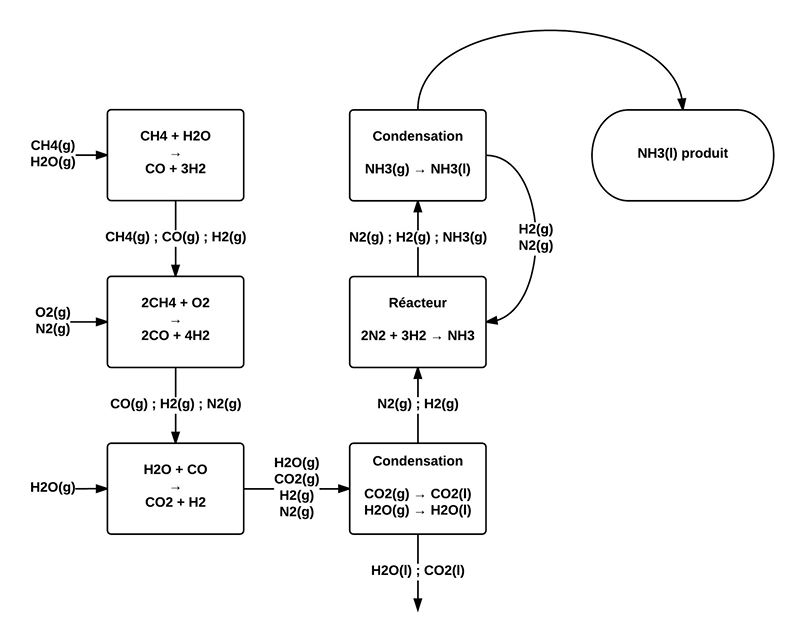
\includegraphics[scale=0.4]{Shema1.jpg}
  	 \caption{Flow-sheet}
  	 \label{Flowsheet}
  \end{center}
\end{figure}


%\end{document}


\end{document}
